\documentclass[pdflatex,sn-mathphys-num]{sn-jnl}
\usepackage{graphicx}
\usepackage{booktabs}
\usepackage{microtype}
\usepackage{amsmath,amssymb}
\usepackage{orcidlink}
\usepackage{needspace}
\usepackage{placeins}
\renewcommand{\orcid}[1]{~\orcidlink{#1}}
\setlength{\bibsep}{0pt}
\renewcommand{\bibfont}{\footnotesize}
\setlength{\textfloatsep}{10pt plus 2pt minus 2pt}
\begin{document}

\title[FABRID-IDS]{FABRID-IDS: Federated Alert-Budget Reallocation for Heterogeneous IoT Intrusion Detection}
\author*[1]{\fnm{Salaheddine} \sur{Naslouby}\orcid{0009-0002-7295-7816}}\email{naslouby.salahe@gmail.com}
\author[2]{\fnm{Mohamed} \sur{Lachgar}}\email{m.lachgar@uca.ac.ma}
\author[1]{\fnm{Hamid} \sur{Hrimech}}\email{hamid.hrimech@uhp.ac.ma}
\affil[1]{\orgname{Hassan First University}, \orgdiv{National School of Applied Sciences (ENSA), LAMSAD Laboratory}, \orgaddress{\city{Berrechid}, \country{Morocco}}}
\affil[2]{\orgname{Cadi Ayyad University}, \orgdiv{Higher Normal School (ENS), L2IS Laboratory}, \orgaddress{\city{Marrakech}, \country{Morocco}}}

\abstract{High pooled attack-ranking performance does not ensure that locally calibrated thresholds meet their nominal false-positive-rate (FPR) targets. FABRID-IDS investigates post-training alert-budget allocation: client-specific nominal rates are selected under a shared weighted constraint, and each threshold is subsequently calibrated on local benign scores. The primary evaluation uses nine N-BaIoT devices, ten detector seeds, and five nominal budgets; CIC IoT-DIAD provides a secondary protocol stress test with different clients, features, and a different scorer. At $B=0.001$, unrestricted Macro and Tail allocations realize a federation FPR of $0.00170$, or $1.696B$, despite satisfying the nominal allocation constraint. Conservative calibration reduces the realized FPR to $0.00036$ but lowers macro recall from $0.3778$ to $0.2445$ and does not restore worst-client recall. Equal-FPR achieves higher macro recall at several nominal budgets, although its realized FPR also exceeds the budget at several operating points. Mean AUROC and AUPRC are $0.9995$ and $0.9999$, yet FABRID-family minimum-client recall remains zero across the evaluated N-BaIoT budgets. The experiments show that satisfying the nominal budget constraint does not ensure control of the realized federation FPR or reliable detection for every client, even when pooled ranking metrics are close to one.}
\keywords{federated intrusion detection, Internet of Things, alert-budget reallocation, false-positive-rate constraint, threshold calibration}
\maketitle

\section{Introduction}\label{sec:introduction}
Federated IoT detection distributes model training across clients, but deployment still requires a threshold that converts anomaly scores into alerts \cite{nguyen2019diot,wang2021noniid,hamdi2023flids}. Shared and client-specific thresholding have been studied \cite{laridi2024threshold,Asiri2025Decentralized,Khan2026FedDTCN}, yet neither determines how a federation-wide FPR budget should be divided across heterogeneous clients. With a frozen scorer, differences in benign-score distributions and attack-recall curves can produce uneven false-alarm and detection-utility outcomes across clients.

FABRID-IDS treats this as alert-budget reallocation. Given a fixed scorer, it uses labeled validation attacks to select client-specific nominal rates $\alpha_k$ under the federation constraint $\sum_k w_k \alpha_k \leq B$. Independent local benign calibration sets the thresholds used for held-out evaluation, allowing us to compare the allocated targets with the observed operating points. $B$ is a nominal federation-level FPR budget, not a realized-FPR guarantee.

We formulate client-specific FPR allocation under a federation-level budget, separate rate selection from final threshold calibration, and evaluate nominal compliance against held-out FPR and recall. The paired N-BaIoT experiments also examine how allocation affects the weakest client, rather than relying only on federation averages.

\section{Related work and scope}\label{sec:related}
Federated IoT IDS research has mainly focused on detector training \cite{nguyen2019diot,wang2021noniid,hamdi2023flids,kairouz2021advances}, while threshold regulation and distributed anomaly detection address related operating-point questions \cite{bridges2017threshold,ochiai2023global}. Laridi et al. \cite{laridi2024threshold} aggregate client summary statistics into one global anomaly threshold. Asiri et al. \cite{Asiri2025Decentralized} compute local 95th-percentile benign reconstruction-error thresholds and average them into one global threshold. Fed-DTCN \cite{Khan2026FedDTCN} uses held-out benign calibration data to select client-specific thresholds for target local FPRs.

Neyman--Pearson classification addresses explicit error-rate constraints \cite{tong2018np}, while conformal calibration provides finite-sample guarantees under specified sampling assumptions \cite{angelopoulos2023gentle}. Federated conformal methods have also examined the effects of predictor sharing and calibration-score aggregation \cite{prism2026fcp}. FABRID-IDS addresses a different decision: how nominal FPR targets should be distributed across clients after the detector has been trained. The allocation is constrained by $\sum_k w_k\alpha_k\leq B$, but thresholds are calculated independently from local benign samples. Lower-tail optimization, order statistics, and finite-sample calibration are established techniques; the contribution here is their use in federation-level rate allocation and the evaluation of the resulting operating points. The method does not guarantee realized-FPR control, and the released N-BaIoT record order does not establish deployment chronology or exchangeability.

Training-time allocation is related but addresses a different decision. Fair federated learning and agnostic federated learning vary how model training responds to client performance or mixtures of clients \cite{kairouz2021advances}. Here the detector is already fixed. Changing $\alpha_k$ changes only the operating threshold used for client $k$; it cannot improve the ordering of benign and attack scores. This separation lets the same scores support paired threshold-policy comparisons, with scorer quality a shared limitation.

A common absolute threshold applies one cutoff across client score distributions. Equal-FPR instead assigns each client the same nominal FPR target but calibrates its threshold locally. FABRID-IDS permits different client targets while constraining their weighted sum. We compare these alternatives using independently calibrated thresholds and held-out scores, so differences between allocated rates and measured operating points can be examined directly.

\section{FABRID-IDS}\label{sec:method}
\subsection{Protocol and utility}
For each client $k$, let $s_k(\cdot)$ denote its frozen anomaly scorer. We divide the released benign records in source order: 50\% for training, 20\% for frontier estimation, 10\% for final calibration, and 20\% for testing. Within each retained attack subtype, the first 20\% of records are assigned to validation and the remainder to testing. Allocation uses the frontier benign scores and validation attacks. Final-calibration and test records are held aside until their respective stages.

For ascending benign scores $x_{(1)},\ldots,x_{(n)}$ and nominal target $\alpha$, threshold calibration uses a standard order-statistic construction \cite{angelopoulos2023gentle}
\begin{equation}
 \tau(\alpha)=x_{(r)},\qquad r=\left\lceil(n+1)(1-\alpha)\right\rceil,
 \label{eq:orderstat}
\end{equation}
with $\tau=+\infty$ if $\alpha\leq0$, $n=0$, or $r>n$; alerts require $s>\tau$. At each candidate rate $\alpha$, frontier benign scores provide a provisional threshold. Applying that threshold to labeled validation attacks gives $u_k(\alpha)$, the mean recall over eligible attack subtypes for client $k$. Allocation therefore depends on attack labels. The grid has 207 candidate rates in $[0,0.05]$, including every evaluated budget. Eligible subtypes require at least 50 validation records, and clients require at least 200 records across two subtypes.

Training records are used to fit the detector and the normalization parameters for each client. After allocation, the provisional frontier threshold is discarded and recalculated using the separate final-calibration benign sample. Test records are reserved for the final evaluation. Frontier estimation and final calibration therefore use disjoint benign observations, although the released source-order partitions may still have different score distributions.

Calibration uses discrete order statistics, so neighboring nominal rates can select the same threshold. Those rates then produce identical decisions on the calibration sample. A change in an allocated $\alpha_k$ consequently need not change the calibrated threshold, held-out FPR, or attack recall. This matters when interpreting the optimizer's selected rates: their numerical differences do not necessarily correspond to different operating points.

For each client, attack recall is averaged across eligible subtypes. Federation macro recall is then calculated as the mean of these client-level values, so clients with more attack records do not receive greater weight. Minimum-client recall is the smallest client-level macro recall. We report both endpoints together with held-out benign FPR, since policies evaluated under the same nominal budget may operate at different measured false-alert rates.

\subsection{Allocation and calibration}
FABRID-IDS reallocates the nominal alert budget by selecting client-specific grid rates subject to
\begin{equation}
 \sum_{k=1}^{K} w_k\alpha_k\leq B. \label{eq:budget}
\end{equation}
Primary N-BaIoT results use $w_k=1/K$, so nominal and realized federation FPR are both equal-client averages. One-hot mixed-integer programs (HiGHS) maximize mean $u_k$ (Macro) or the mean of the lowest $q=\lceil0.25K\rceil$ client utilities (Tail) \cite{rockafellar2000cvar}. For $K=9$ and $q=3$, Tail maximizes the mean of the three lowest client utilities, unlike conventional empirical CVaR at tail fraction 0.25, which assigns fractional weight to the third client \cite{rockafellar2000cvar}. Minimum-client recall is reported separately. For a frontier benign sample containing $n_f$ records, positive candidate rates below $2/(n_f+1)$ are excluded, matching the zero-calibration-alert transition under strict thresholding.

Equal-client weighting makes federation FPR the mean of device-level rates rather than the proportion of flagged records in the pooled benign dataset. Pooling would give more weight to devices with larger retained samples, although the samples do not establish comparable traffic durations. The budget constraint is an upper bound; some budget may remain unused, and individual clients may receive a zero target. Macro maximizes estimated mean recall, then minimizes nominal expenditure among solutions meeting the primary objective within solver tolerances. Tail first maximizes the mean utility of the three weakest clients, followed by estimated mean utility and nominal expenditure. Both programs use estimated utility variance and deterministic tie-breaking for the remaining choices. Macro and Tail derive their allocations from frontier scores and validation attacks, without consulting final-calibration or test records. Equal-FPR assigns the same nominal target to each client. Under ordinary calibration, Macro, Tail, and Equal-FPR use the same benign samples and the order-statistic rule in Eq.~\eqref{eq:orderstat}. The conservative Macro and Tail variants use those same samples but select their thresholds through Eq.~\eqref{eq:conservative}.

Tail optimizes the average utility of the three lowest-performing clients, not the minimum utility itself. Gains for two of those clients can therefore increase the objective even when the third continues to detect no attacks.

Final thresholds are recalibrated with Eq.~\eqref{eq:orderstat}. The conservative intervention selects the smallest rank satisfying the binomial calibration construction \cite{tong2018np}
\begin{equation}
 r_{.95}=\min\{r:\Pr[\mathrm{Binomial}(n,1-\alpha)\leq r-1]\geq0.95\}.
 \label{eq:conservative}
\end{equation}
Equation~\eqref{eq:conservative} searches the ranks from $1$ through $n$ and selects $x_{(r_{.95})}$ when a qualifying rank exists. Otherwise, the threshold is set to $+\infty$, as it is when $n=0$ or $\alpha=0$. Alerts continue to require $s>\tau$. Under independent, identically distributed benign calibration and future scores, the binomial criterion supplies a one-sided 95\% confidence statement about the client's population FPR. It does not constrain the measured FPR on an arbitrary fixed test partition. We therefore evaluate this rule as a finite-sample sensitivity intervention, without claiming its nominal guarantee holds for the released source-order split.

The conservative rule usually selects a higher threshold than the ordinary order statistic, reducing benign alerts but potentially losing attack detections. Its binomial criterion accounts for calibration uncertainty under the stated sampling assumptions; the ordinary rule uses the rank specified by Eq.~\eqref{eq:orderstat}. Neither rule adjusts its threshold using test outcomes or corrects a difference between calibration and future score distributions.

An observed FPR above the assigned target does not imply that the nominal allocation violated Eq.~\eqref{eq:budget}. Conversely, a low test FPR does not establish control under different traffic conditions. We therefore distinguish four quantities: the allocated client rate, the selected calibration rank, calibration-sample FPR, and held-out FPR. Equal-FPR and the optimized policies use the same final-calibration procedure, leaving rate assignment as the policy difference examined in the experiment.

With strict alerts, $\alpha<2/(n+1)$ gives either $r>n$ or a maximum-score threshold and zero calibration alerts; the smallest nonzero empirical FPR is $1/n$ (absent ties). Rates below this transition cannot generate a nonzero empirical calibration FPR under strict thresholding; excluding them prevents the optimizer from assigning nominal budget to grid points that are empirically indistinguishable from a zero-alert calibration point. Ecobee has $n=1311$ on the final-calibration split, so targets below $0.001524$ calibrate to zero alerts. This calculation explains why sufficiently small allocated rates produce no calibration alerts, but it does not explain the subsequent held-out FPR shift.

\subsection{Frozen scorer}
The primary scorer is the maximum of frozen frontier-reference percentile ranks for autoencoder reconstruction error and the jitter-based temporal feature \texttt{HH\_jit\_L0.1\_mean} ($f_{75}$). The $f_{75}$ candidate and scorer configuration were selected through predeclared development-only ablations. The autoencoder uses [64,16] layers and is trained over ten federated rounds, with three local epochs per round. Training uses row-count-weighted averaging, Adam with learning rate 0.001, batch size 64, mean squared error, and normalization fitted separately on each client's training split. Ten detector seeds provide the paired replication units. Both score components are transformed into percentile ranks against frozen frontier references before their maximum is taken. AUROC and AUPRC remain unchanged across policies because each policy uses the same frozen scores; only the selected threshold differs.

\section{Experimental methodology}\label{sec:experiments}
The primary experiment uses nine N-BaIoT devices and five prespecified budgets from $B=0.001$ through $B=0.020$ (Table~\ref{tab:primary}). Macro recall is the mean of client-level macro recalls over eligible attack subtypes; minimum-client recall is their minimum.

N-BaIoT contains benign traffic and BASHLITE and Mirai attack records from commercial IoT devices \cite{meidan2018nbaiot}. The nine devices are natural clients in this study. Their benign sample sizes are unequal, ranging from 13,113 records for Ecobee to 175,240 for the Philips baby monitor in the retained data. After the source-order split, the final-calibration sample is correspondingly small for Ecobee. This imbalance makes an equal nominal rate a different empirical threshold problem on different devices even before the attack-score distributions are considered.

The five nominal budgets are $0.001$, $0.0025$, $0.005$, $0.010$, and $0.020$. Within each seed, policies are evaluated using the same trained detector and score partitions. Policy differences are therefore paired by seed; individual test records are not treated as independent experimental replicates. The reported means describe the fixed benchmark and its ten detector seeds rather than performance over independently sampled devices or collection periods.

Each reported federation FPR is computed from the held-out benign FPR of each device with the same equal-client weights as the nominal constraint. The test is not an independent draw from the calibration distribution: the released records are ordered and their traffic features use overlapping windows, and seed replication reflects detector variation rather than resampling of collection periods or devices.

The prespecified contrasts compare Macro with Equal-FPR on macro recall and Tail with Equal-FPR on minimum-client recall. Each comparison uses ten paired detector seeds, exact sign-flip testing, 50,000 paired-bootstrap resamples, and Holm correction across the five budgets.

Statistical inference uses the detector seed as the unit of replication. For each budget, client outcomes are first aggregated into the specified endpoint, yielding ten paired policy differences. The two-sided exact sign-flip test enumerates $2^{10}=1{,}024$ possible sign assignments. Pointwise 95\% confidence intervals are obtained from 50,000 bootstrap resamples of the paired seed differences. Holm correction is applied to the five budget-wise $p$-values within each endpoint family, not to the confidence intervals. These calculations characterize variation across detector seeds on the fixed data partitions; they do not estimate uncertainty for independently collected traffic or unseen devices.

CIC IoT-DIAD is drawn from the device-identification and anomaly-detection study of Rabbani et al. \cite{rabbani2025iotdiad}. It contributes 19 physical-device clients and 57 features. A new detector is trained for this dataset using reconstruction-error scores alone; no N-BaIoT checkpoint is transferred. The benign partition proportions and attack-validation fraction follow the primary protocol. Because the client population, feature representation, and scorer differ from N-BaIoT, this experiment cannot identify which component accounts for any difference between the datasets.

\section{Results}\label{sec:results}
\subsection{Nominal and realized operating points}
At $B=0.001$, unrestricted Macro and Tail both produce a realized federation FPR of $0.00170$ ($1.696B$). Their conservative variants reduce it to $0.00036$ ($0.358B$), while macro recall falls from $0.3778$ to $0.2445$. All four allocations satisfy the same nominal budget ceiling, but the realized FPR is measured independently on held-out benign records after local calibration.

\Needspace{9\baselineskip}
The size of the mismatch varies across budgets and policies. At $B=0.0025$, Macro and Tail have a measured FPR of approximately $1.03B$, whereas Equal-FPR also exceeds its nominal target at several other budgets. Budget overshoot is not confined to optimized allocations. Figure~\ref{fig:realized}(b) shows macro recall against realized federation FPR.
\begin{figure}[tbp]
\centering
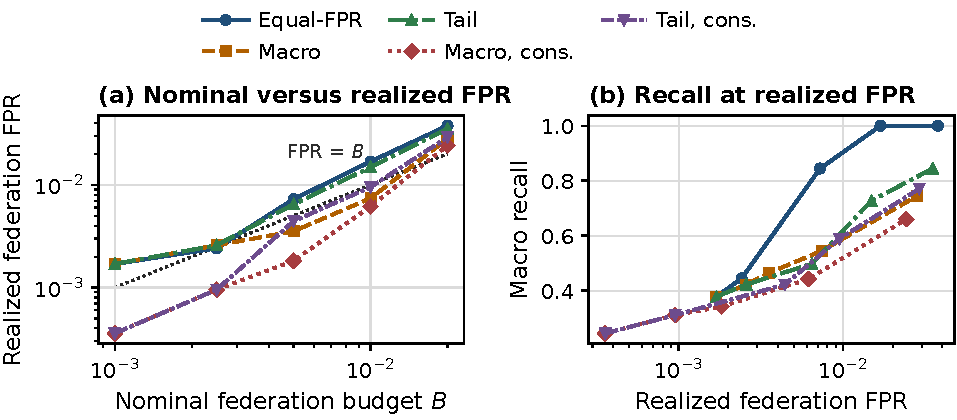
\includegraphics[width=0.7\textwidth]{realized_fpr_lines.pdf}
\caption{N-BaIoT ten-seed means: realized FPR versus nominal budget (left) and macro recall versus realized FPR (right). The diagonal marks equal rates.}
\label{fig:realized}
\end{figure}

At $B=0.005$, Equal-FPR reaches macro recall $0.8444$ at a realized FPR of $1.45B$. Macro reaches $0.4644$ at $0.71B$, while Tail reaches $0.4977$ at $1.29B$. At $B=0.020$, Equal-FPR reaches recall $1.0000$, compared with $0.7444$ for Macro and $0.8444$ for Tail. The corresponding realized FPR ratios are $1.88B$, $1.40B$, and $1.75B$. Equal-FPR has higher recall at these budgets, but at different measured FPRs.

\begin{table}[tbp]
\caption{N-BaIoT ten-seed means. Each policy cell reports macro recall; realized federation FPR divided by nominal budget. All FABRID-family cells have zero minimum-client recall.}
\label{tab:primary}
\centering
\small
\renewcommand{\arraystretch}{1.00}
\begin{tabular*}{\textwidth}{@{\extracolsep{\fill}}lccccc@{}}
\toprule
$B$ & Equal-FPR & Macro & Tail & Macro, cons. & Tail, cons.\\
\midrule
0.0010 & 0.3778; 1.70 & 0.3778; 1.70 & 0.3778; 1.70 & 0.2445; 0.36 & 0.2445; 0.36\\
0.0025 & 0.4445; 0.97 & 0.4222; 1.03 & 0.4222; 1.03 & 0.3111; 0.38 & 0.3111; 0.38\\
0.0050 & 0.8444; 1.45 & 0.4644; 0.71 & 0.4977; 1.29 & 0.3422; 0.36 & 0.4222; 0.88\\
0.0100 & 0.9999; 1.68 & 0.5444; 0.74 & 0.7266; 1.48 & 0.4422; 0.62 & 0.5889; 0.95\\
0.0200 & 1.0000; 1.88 & 0.7444; 1.40 & 0.8444; 1.75 & 0.6600; 1.21 & 0.7711; 1.45\\
\bottomrule
\end{tabular*}
\end{table}

We examined the stability of Macro allocations by resampling frontier benign scores and validation attack scores before resolving the allocation problem. Each seed and budget uses 500 bootstrap replicates, resampled within subtype, that rerun unrestricted Macro allocation; the scorer, final-calibration scores, and test scores stay fixed. Within each seed--client--budget cell, a change means that the selected rate differs from the modal rate among its 500 replicates. Averaging those change frequencies over ten seeds and nine clients gives 77.8, 79.8, 83.9, 83.6, and 84.9\% at the five ascending budgets. These are means of 90 cell-level frequencies per budget, not a count of seeds with any change. They measure sensitivity to resampled allocation evidence, not changes relative to the original allocation or repeated deployments.

\begin{figure}[tbp]
\centering
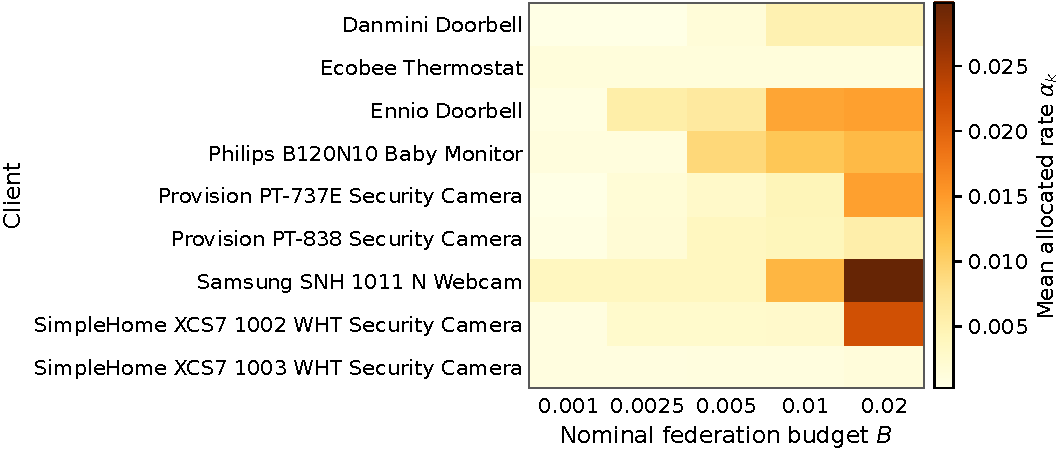
\includegraphics[width=0.75\textwidth]{macro_allocation_heatmap.pdf}
\caption{Original unrestricted Macro rates $\alpha_k$, averaged across ten N-BaIoT seeds. The heatmap excludes the 500 frontier resamples.}
\label{fig:allocation}
\end{figure}

\Needspace{6\baselineskip}
Figure~\ref{fig:allocation} shows how Macro distributes the nominal budget unevenly across the nine devices. At $B=0.020$, the largest mean allocations go to the Samsung webcam and the SimpleHome XCS7 1002 camera, while Danmini receives a comparatively small allocation. The heatmap contains the original allocations averaged across ten detector seeds; the 500 frontier resamples contribute only to the sensitivity analysis reported above.

\subsection{Tail objective and worst-client behavior}
Tail optimizes the rounded three-client lower-tail mean, but minimum-client recall is zero for every FABRID policy--budget cell and cannot distinguish unrestricted Macro and Tail. Danmini Doorbell has zero macro attack recall under every evaluated unrestricted-policy operating point; its final-calibration and held-out benign FPR are also zero in all 100 unrestricted-policy--seed--budget cells. With $n=4955$ benign final-calibration records, its zero-alert transition is $2/(n+1)=0.000404$; its allocated-rate range crosses this finite-sample transition.

Unlike Danmini, Ecobee produces held-out benign alerts despite having none in its final-calibration sample. At $B=0.020$, Macro assigns Ecobee a mean nominal rate of $0.001164$. Its measured benign FPR is $0.006672$, with macro attack recall of $0.6000$. Danmini, by comparison, has zero held-out benign FPR and zero attack recall under the evaluated unrestricted policies.

Ecobee has 1,311 benign final-calibration records, compared with 4,955 for Danmini. The different sample sizes affect the resolution of their order-statistic thresholds, but cannot alone explain the observed test outcomes. In particular, zero calibration alerts need not imply zero false alarms on held-out records. The released source-order partitions do not permit the discrepancy to be attributed to calibration resolution or distributional differences individually.

\Needspace{10\baselineskip}
\subsection{Primary contrasts and ranking ceiling}
Macro and Equal-FPR are identical at $B=0.001$; their $-0.0222$ difference at $B=0.0025$ is not statistically distinguishable from zero, and Macro recall is lower at larger budgets. Both Tail and Equal-FPR have zero mean minimum-client recall through $B=0.005$. At $B=0.010$ and $0.020$, Equal-FPR reaches $0.9998$ and $0.9999$ minimum-client recall while Tail remains at zero (Table~\ref{tab:contrasts}); Equal-FPR's realized FPR is also $1.68B$ and $1.88B$ at those budgets.

\begin{table}[tbp]
\caption{Prespecified paired seed-level contrasts ($n=10$): 50,000 paired-bootstrap CIs and Holm-adjusted exact paired sign-flip $p$ values over the five-budget family.}
\label{tab:contrasts}
\centering
\small
\renewcommand{\arraystretch}{1.00}
\setlength{\tabcolsep}{4pt}
\begin{tabular*}{\textwidth}{@{\extracolsep{\fill}}lcccccc@{}}
\toprule
& \multicolumn{3}{c}{Macro $-$ Equal-FPR: macro recall} & \multicolumn{3}{c}{Tail $-$ Equal-FPR: minimum-client recall}\\
\cmidrule(lr){2-4}\cmidrule(l){5-7}
$B$ & Mean $\Delta$ & 95\% CI & Holm $p$ & Mean $\Delta$ & 95\% CI & Holm $p$\\
\midrule
0.0010 & 0.0000 & [0.0000, 0.0000] & 1.0000 & 0.0000 & [0.0000, 0.0000] & 1.0000\\
0.0025 & $-$0.0222 & [$-$0.0556, 0.0111] & 0.3594 & 0.0000 & [0.0000, 0.0000] & 1.0000\\
0.0050 & $-$0.3800 & [$-$0.4133, $-$0.3466] & 0.0098 & 0.0000 & [0.0000, 0.0000] & 1.0000\\
0.0100 & $-$0.4555 & [$-$0.5000, $-$0.4111] & 0.0098 & $-$0.9998 & [$-$0.9998, $-$0.9998] & 0.0098\\
0.0200 & $-$0.2556 & [$-$0.2889, $-$0.2222] & 0.0098 & $-$0.9999 & [$-$0.9999, $-$0.9999] & 0.0098\\
\bottomrule
\end{tabular*}
\end{table}

Because allocation changes thresholds rather than anomaly scores, AUROC and AUPRC are policy-invariant by construction. For each detector seed, the implementation pools held-out benign scores across all nine clients and attack-test scores across subtypes, then computes a rank-based AUROC and a trapezoidal precision--recall area. The reported $0.9995$ AUROC and $0.9999$ AUPRC are means of these pooled values over ten seeds, not of client-level areas, with attack subtypes and clients weighted by held-out row count. From the retained counts and split boundaries, the test pool has 1,041,078 attack and 111,188 benign rows (90.35\% attack prevalence), which raises the AUPRC reference level. Pooling scores across devices makes the resulting ranking metrics dependent on the number of retained test records per device and subtype. Neither area establishes strong ranking for every client, nor does it describe performance at an individual calibrated threshold. Nevertheless, minimum-client recall remains zero for every FABRID-family policy at all five N-BaIoT budgets.

Table~\ref{tab:contrasts} compares policies at fixed nominal budgets, not at matched realized FPR. Its intervals summarize the paired seed differences on the fixed split, while the adjusted $p$-values account for the specified budget-wise comparisons. Neither changes the measured FPR at which recall was obtained. Figure~\ref{fig:realized} connects the five evaluated operating points; estimating recall differences at a common measured FPR would require a separate matching procedure.


\subsection{Secondary protocol stress test}
CIC IoT-DIAD provides a secondary protocol stress test of unrestricted Macro allocation with ordinary local order-statistic calibration. Table~\ref{tab:external} averages held-out evaluations over ten independently trained detector seeds, with 19 equally weighted physical-device clients and reconstruction-error scoring. The benign splits and attack-validation fraction match N-BaIoT; each seed trains a new detector, and no N-BaIoT weights or score rankings are transferred. Across the five nominal budgets, macro recall ranges from $0.3614$ to $0.5016$, realized federation FPR from $0.0098$ to $0.0311$, and minimum-client recall from $0.0000$ to $0.0251$.

\begin{table}[!htbp]
\caption{CIC IoT-DIAD: unrestricted Macro with ordinary local calibration; ten-seed means over 19 equally weighted clients using reconstruction-error scores.}
\label{tab:external}
\centering
\renewcommand{\arraystretch}{1.00}
\begin{tabular*}{0.82\textwidth}{@{\extracolsep{\fill}}lccc@{}}
\toprule
$B$ & Macro recall & Minimum-client recall & Realized FPR\\
\midrule
0.0010 & 0.3614 & 0.0000 & 0.0098\\
0.0025 & 0.3970 & 0.0000 & 0.0118\\
0.0050 & 0.4318 & 0.0007 & 0.0160\\
0.0100 & 0.4602 & 0.0089 & 0.0213\\
0.0200 & 0.5016 & 0.0251 & 0.0311\\
\bottomrule
\end{tabular*}
\end{table}

The realized federation FPR also exceeds the nominal budget in this dataset, but different clients, features, and scoring prevent attribution to the same mechanism as in N-BaIoT. Across the five budgets, the secondary realized FPR is $9.80$, $4.72$, $3.20$, $2.13$, and $1.56$ times the respective nominal ceiling. The decreasing FPR-to-budget ratios should not be confused with a reduction in false alarms. As $B$ rises from $0.001$ to $0.020$, the measured federation FPR increases from $0.0098$ to $0.0311$, while minimum-client recall reaches only $0.0251$. Equal-FPR was not evaluated on these 19 clients under the same detector protocol. Consequently, the secondary results establish budget overshoot for Macro but cannot determine whether it improves the recall--FPR trade-off over a common nominal client rate.

\FloatBarrier
\section{Discussion}\label{sec:discussion}
On N-BaIoT, nominal budget feasibility does not imply realized budget fidelity. Equal-FPR achieves higher macro recall at several budgets, so the evidence does not support uniform superiority of any allocation policy.

Equation~\eqref{eq:budget} constrains the allocated nominal rates before final calibration, not the number of false alerts subsequently observed. At small budgets, conservative calibration can sharply reduce benign alerts while also suppressing attack detections. Danmini remains undetected under the evaluated policies despite these changes in threshold selection. This is a limitation of the resulting operating points, not a violation of the nominal optimization constraint.

Macro and Tail estimate client utility from validation attack recall at provisional frontier thresholds. Final thresholds instead use separate benign calibration samples. Ecobee demonstrates that zero calibration alerts can coexist with nonzero held-out benign FPR, but the source-order partition does not establish that temporal drift caused the discrepancy. Because the utility curves require labeled validation attacks, FABRID-IDS is an attack-informed post-training allocation method rather than a label-free adaptive detector.

Across the five budgets, recorded solver times range from 95.7 to 358.8 ms for Macro and from 310.3 to 3883.1 ms for Tail, without a recorded fallback. These figures cover optimization rather than end-to-end operation. They exclude communication, score generation, calibration transfer, and alert handling.

The primary evaluation uses one hybrid scorer, nine N-BaIoT devices, ten seeds, and five nominal budgets. The secondary evaluation changes the clients, features, and scorer simultaneously. Although both datasets exhibit nominal-to-realized FPR mismatch, these experiments cannot isolate a common cause. Establishing one would require controlled comparisons that vary those components separately. The study also does not evaluate adversarial clients, privacy guarantees, end-to-end deployment overhead, or modifications to the scorer intended to recover missed attacks.


At $B=0.020$, Equal-FPR attains higher macro recall than Macro, but its realized FPR is also higher: $1.88B$ versus $1.40B$ (Table~\ref{tab:primary}). The comparison favors Equal-FPR at that nominal budget; it does not establish which policy would achieve higher recall at the same measured false-alert rate.

With ten paired seeds, the two-sided exact sign-flip test enumerates $2^{10}=1{,}024$ sign assignments. When all ten paired differences are nonzero and share one sign, the smallest raw $p$-value is $2/1{,}024=0.001953125$. Holm adjustment across the five budgets gives $0.0098$, the smallest adjusted value reported in Table~\ref{tab:contrasts}. At $B=0.001$, identical policy outcomes yield $p=1$ and a zero-width confidence interval. The minimum-client intervals at $B=0.010$ and $B=0.020$ are nearly degenerate because Tail recall is zero in every seed and Equal-FPR recall varies only beyond the fourth decimal. The Holm adjustments cover each endpoint's five-budget family separately; they do not correct across both endpoints.

Equation~\eqref{eq:conservative} provides a per-client population-FPR statement under i.i.d. benign calibration and future scores. Even if those assumptions held for all nine N-BaIoT clients, a union bound would give only a conservative lower bound of $1-9(0.05)=0.55$ for simultaneous satisfaction of their nominal FPR targets. This per-client construction has not been validated as a federation-level guarantee on the released data.

A site requiring a hard federation-level FPR ceiling needs more than the nominal constraint in Eq.~\eqref{eq:budget}. The calibration sample must represent the benign traffic on which future decisions will be made, and the achieved FPR must be checked after threshold selection. At the tightest N-BaIoT budget, conservative calibration reduced measured false positives but also lowered recall without recovering Danmini's attack detections. Sustained error-rate control would require an independently justified calibration and monitoring procedure.

The policy comparisons share the same frozen scores within each seed, but their selected rates produce different measured false-alert rates. Recall differences at a fixed nominal budget therefore combine rate allocation with the operating point achieved after calibration. Tail introduces a separate distinction: improving the mean utility of the three weakest clients does not necessarily improve the single worst client. These findings favor reporting allocated rates, realized FPR, macro recall, and minimum-client recall together. Paired seeds control detector variation within the benchmark; independent traffic collections and repeated calibration samples would be necessary to assess whether the observed operating points persist elsewhere.

\section{Conclusion}\label{sec:conclusion}
FABRID-IDS divides a nominal federation-level FPR budget among clients and calibrates the resulting thresholds on local benign scores. On N-BaIoT, feasible nominal allocations did not consistently produce held-out false-positive rates within the specified budget. At $B=0.001$, Macro and Tail yielded a realized federation FPR of $0.00170$; conservative calibration reduced it to $0.00036$ but lowered attack recall. Equal-FPR achieved higher macro recall at several budgets, while minimum-client recall remained zero under the FABRID-family policies. CIC IoT-DIAD also exhibited nominal-to-realized mismatch, although the secondary experiment lacked a matched Equal-FPR baseline. These results establish the limits of nominal rate allocation under the evaluated calibration protocol, not a general performance advantage for reallocation. Future work should examine deployment-ordered calibration and methods that explicitly control realized FPR. The implementation and reproducibility artifacts are available at \url{https://doi.org/10.5281/zenodo.22113172}. The authors declare no competing interests.

\bibliography{references}
\end{document}
